\section{Accessibilità}
\subsection{Separazione tra contenuto, presentazione e struttura}
Per migliorare l'accesso al sito da parte degli utenti con differenti disabilità e per aiutare i motori di ricerca è stata mantenuta la separazione tra struttura, presentazione e comportamento.
La prima è stata sviluppata tramite documenti XHTML Strinct 1.0 e HTML5, i quali richiamano i fogli di stile esterni CSS che implementano la presentazione.
Infine script esterni realizzati con PHP che formano il comportamento e script Javascript per il controllo dei dati inseriti.
\subsection{Screen reader}
Ogni foto di contenuto è stata arricchita di attributi alt contenenti una descrizine esaustiva dell'immagine.
Ogni campo di un form è stato corredato con una etichetta label e le varie voci sono state raggruppate in filedset.
\subsection{Colori}
I colori scelti per il sito hanno un contrato abbastanza elevato per facilitare la lettura dei contenuti alle persone che soffrono di disturbi visivi come il daltonismo.
Il sito è steso in bianco, grigio e nero, con elementi di navigazione evidenziati in rosso.
Per evitare di confondere gli utenti i link vengono sempre rappresentati con sottolineatura e di colore diverso a seconda che il sia stato visitato o mneo, fatta eccezione del menù di navigazione.
In esso lo sfondo rosso indica la pagina aperta e i link alle altre pagine si notano al pasaggio del mouse cambiando il colore della casella da grigio a nero.
Per essere sicuri di aver scelto dei colori che non creino problemi o confusione, è stata testata la homepage utilizzando il servizio offerto dal sito \underline{\color{Blue}http://www.color-blindness.com}.
Questo sito permette infatti di visualizzare la pagina come vista da persone con detrminati disturbi visivi.
Di seguito sono riportati dei test eseguiti sulla pagina della prenotazione camere:

\begin{figure}[htbp]
	\centering
	\begin{minipage}[c]{.40\textwidth}
		%\centering\setlength{\captionmargin}{0pt}%
		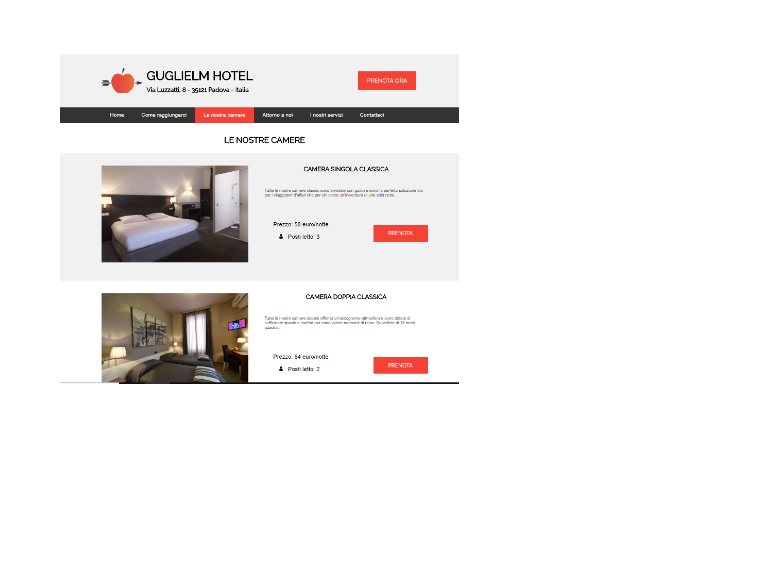
\includegraphics[width=.70\textwidth]{../templates/_Immagini/normal.png}
		\caption{vista normale}
	\end{minipage}%
	\hspace{10mm}%
	\begin{minipage}[c]{.40\textwidth}
		%\centering\setlength{\captionmargin}{0pt}%
		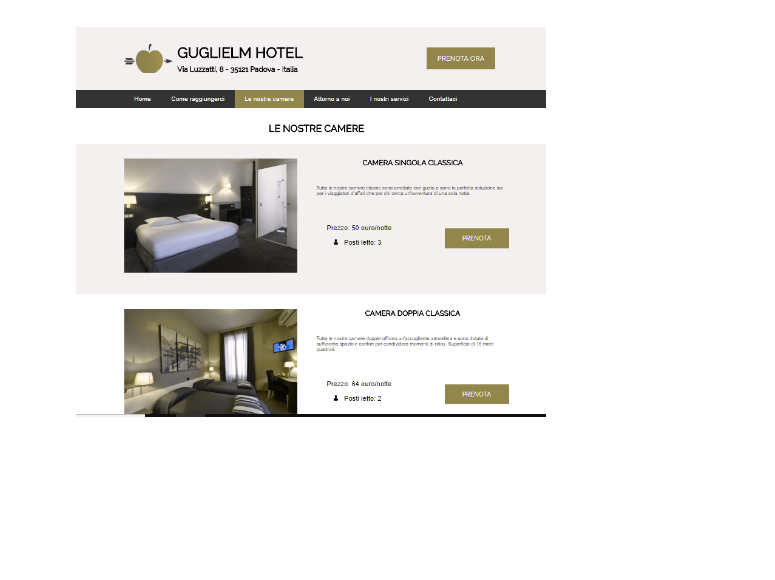
\includegraphics[width=.70\textwidth]{../templates/_Immagini/pranatopia.png}
		\caption{vista da un affetto da pranatopia}
	\end{minipage}
\end{figure}

\begin{figure}[htbp]
	\centering
	\begin{minipage}[c]{.40\textwidth}
		%\centering\setlength{\captionmargin}{0pt}%
		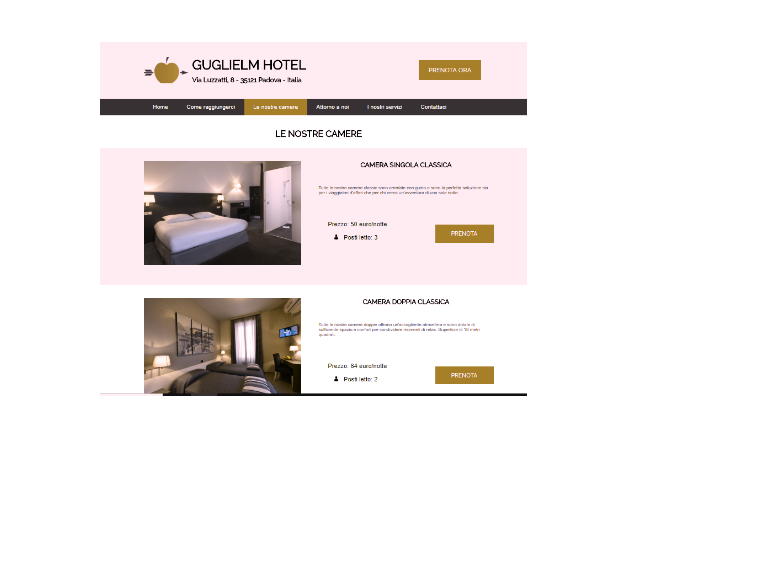
\includegraphics[width=.70\textwidth]{../templates/_Immagini/deut.png}
		\caption{vista da un affetto da deutanotopia}
	\end{minipage}%
	\hspace{10mm}%
	\begin{minipage}[c]{.40\textwidth}
		%\centering\setlength{\captionmargin}{0pt}%
		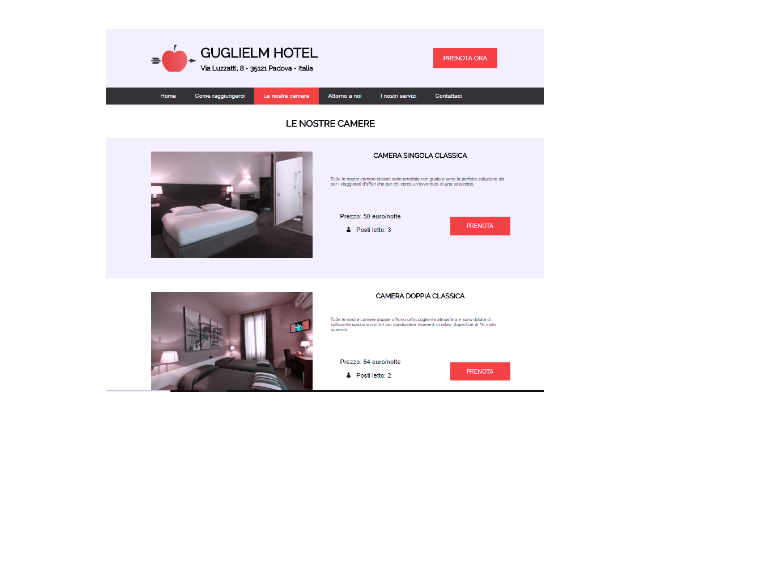
\includegraphics[width=.70\textwidth]{../templates/_Immagini/trita.png}
		\caption{vista da un affetto da tritanotopia}
	\end{minipage}
\end{figure}



